\begin{figure}[t]
    % First row
    \centering
    \begin{subfigure}{0.46\textwidth}
        \centering
        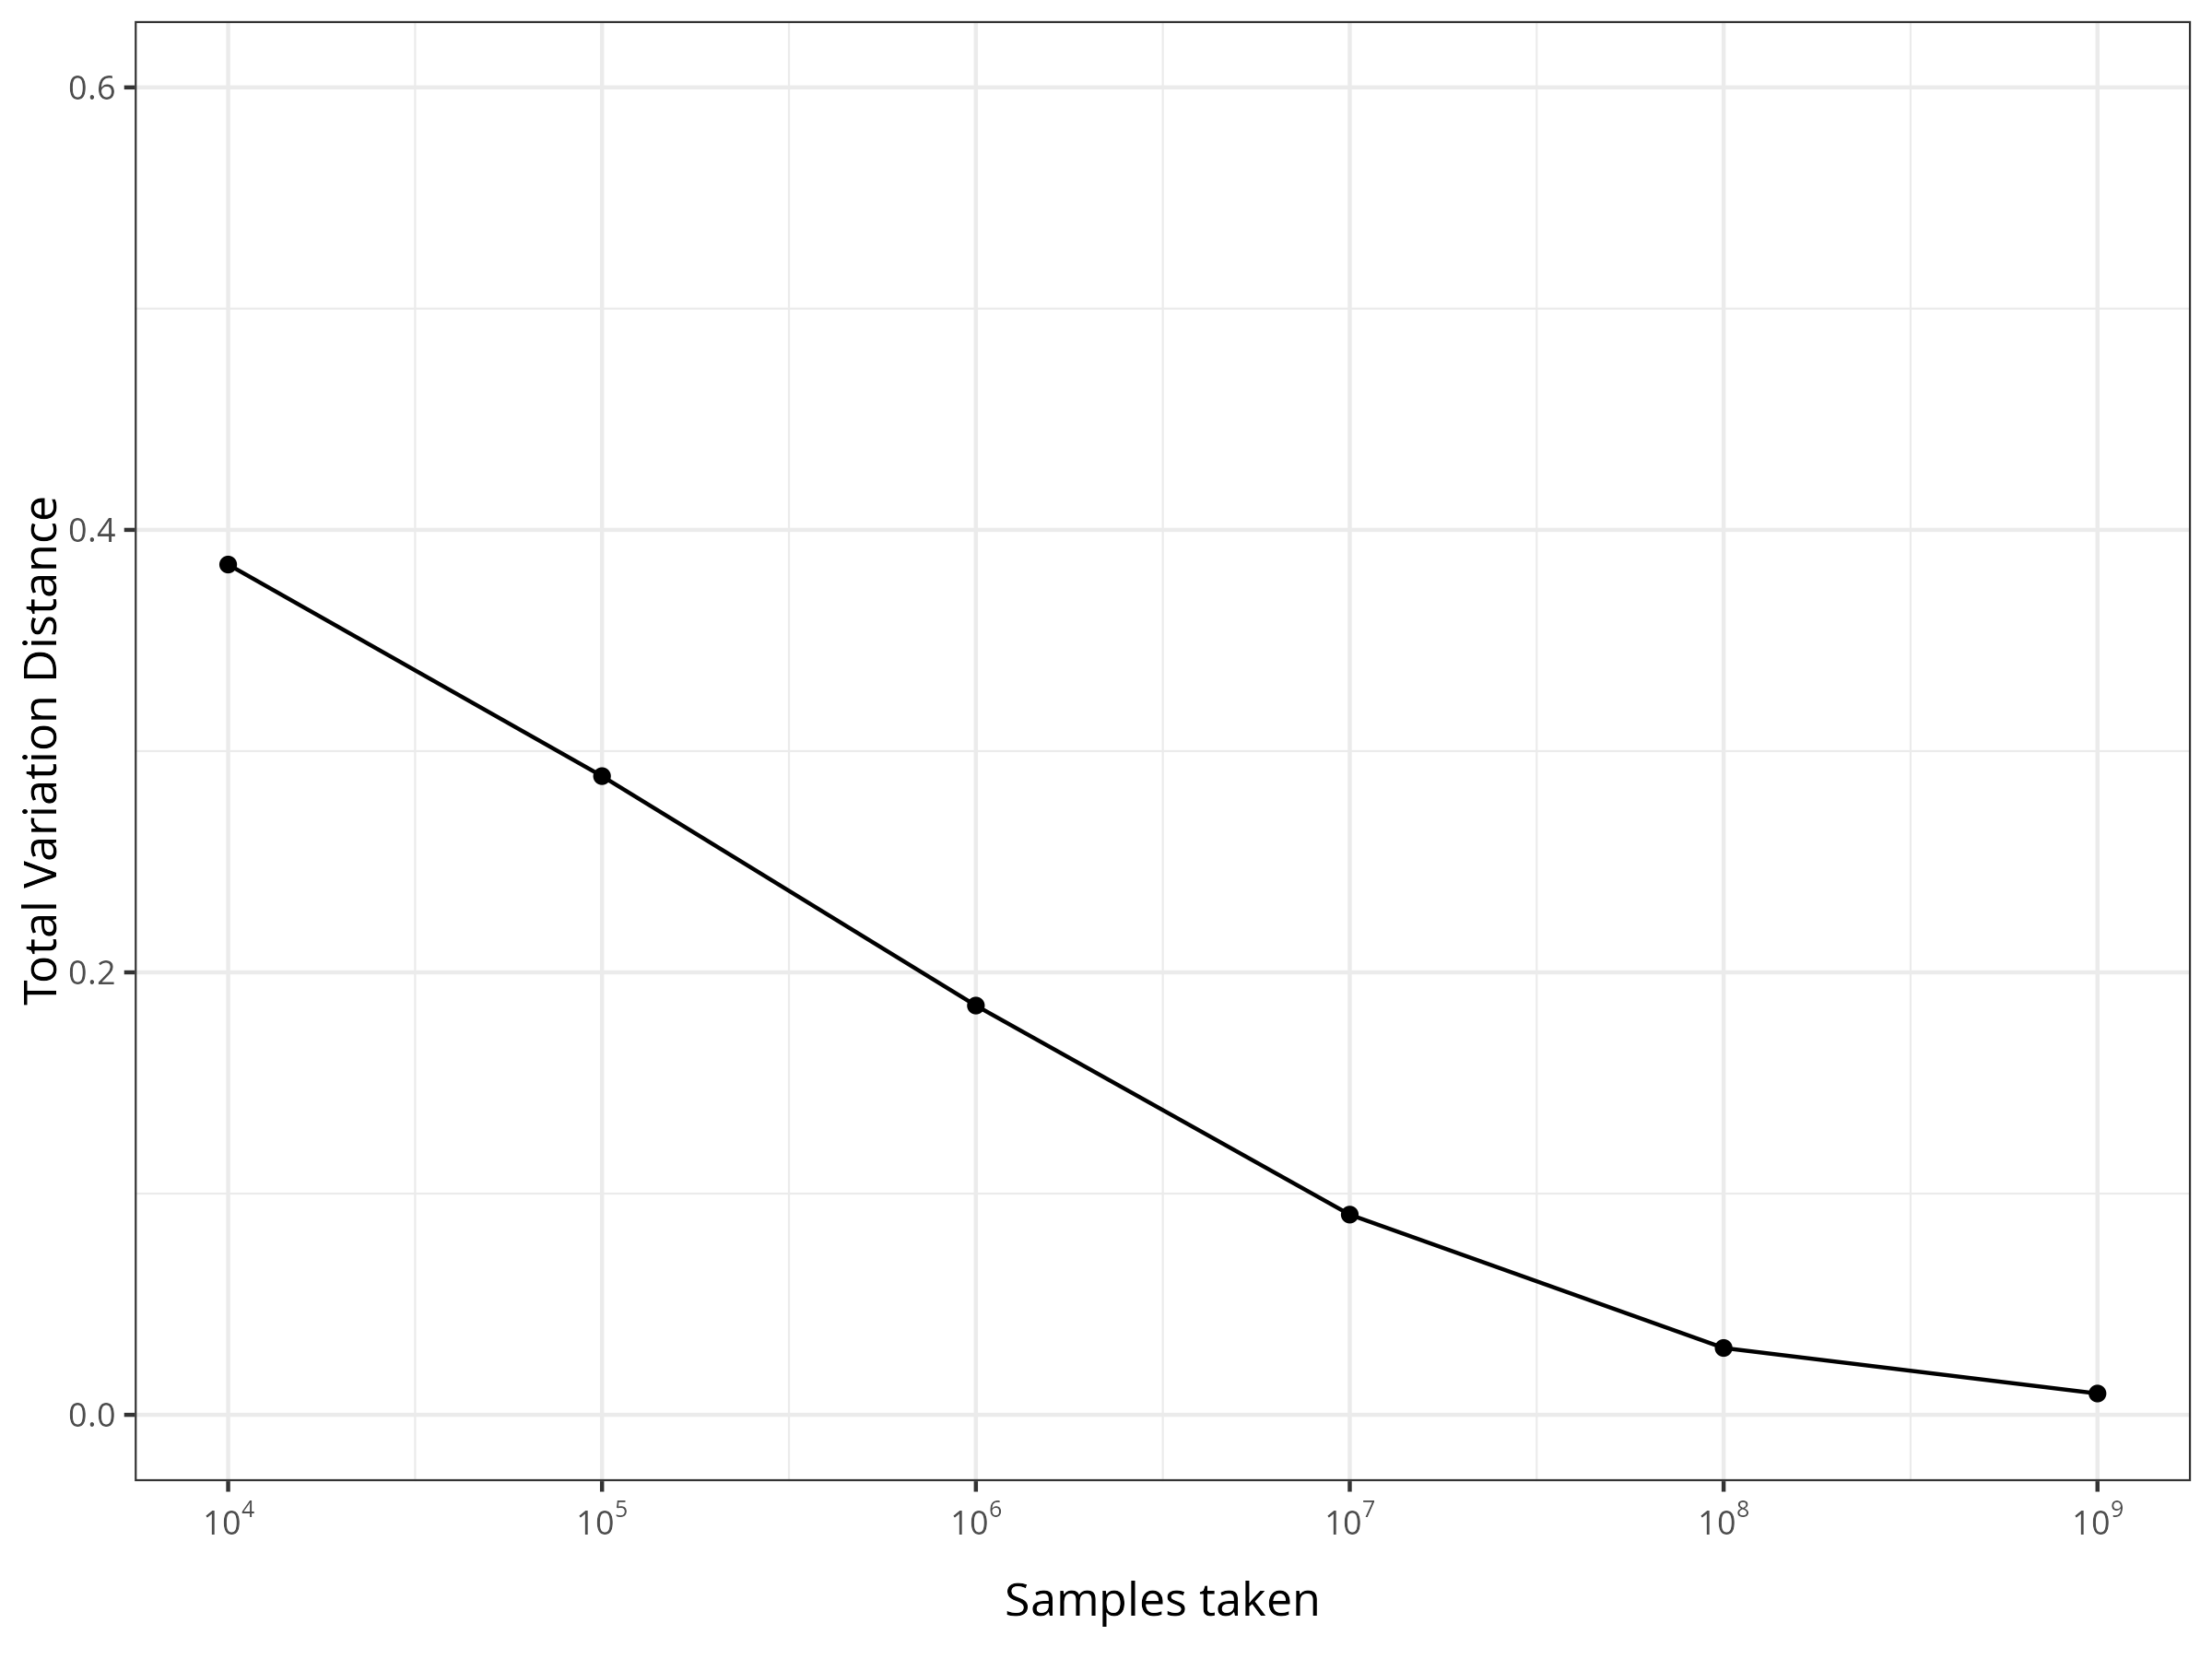
\includegraphics[width=\textwidth]{figures/tvd/apache.png}
        \caption{Rejection-Inversion}
    \end{subfigure}
    \hfill
    \begin{subfigure}{0.46\textwidth}
        \centering
        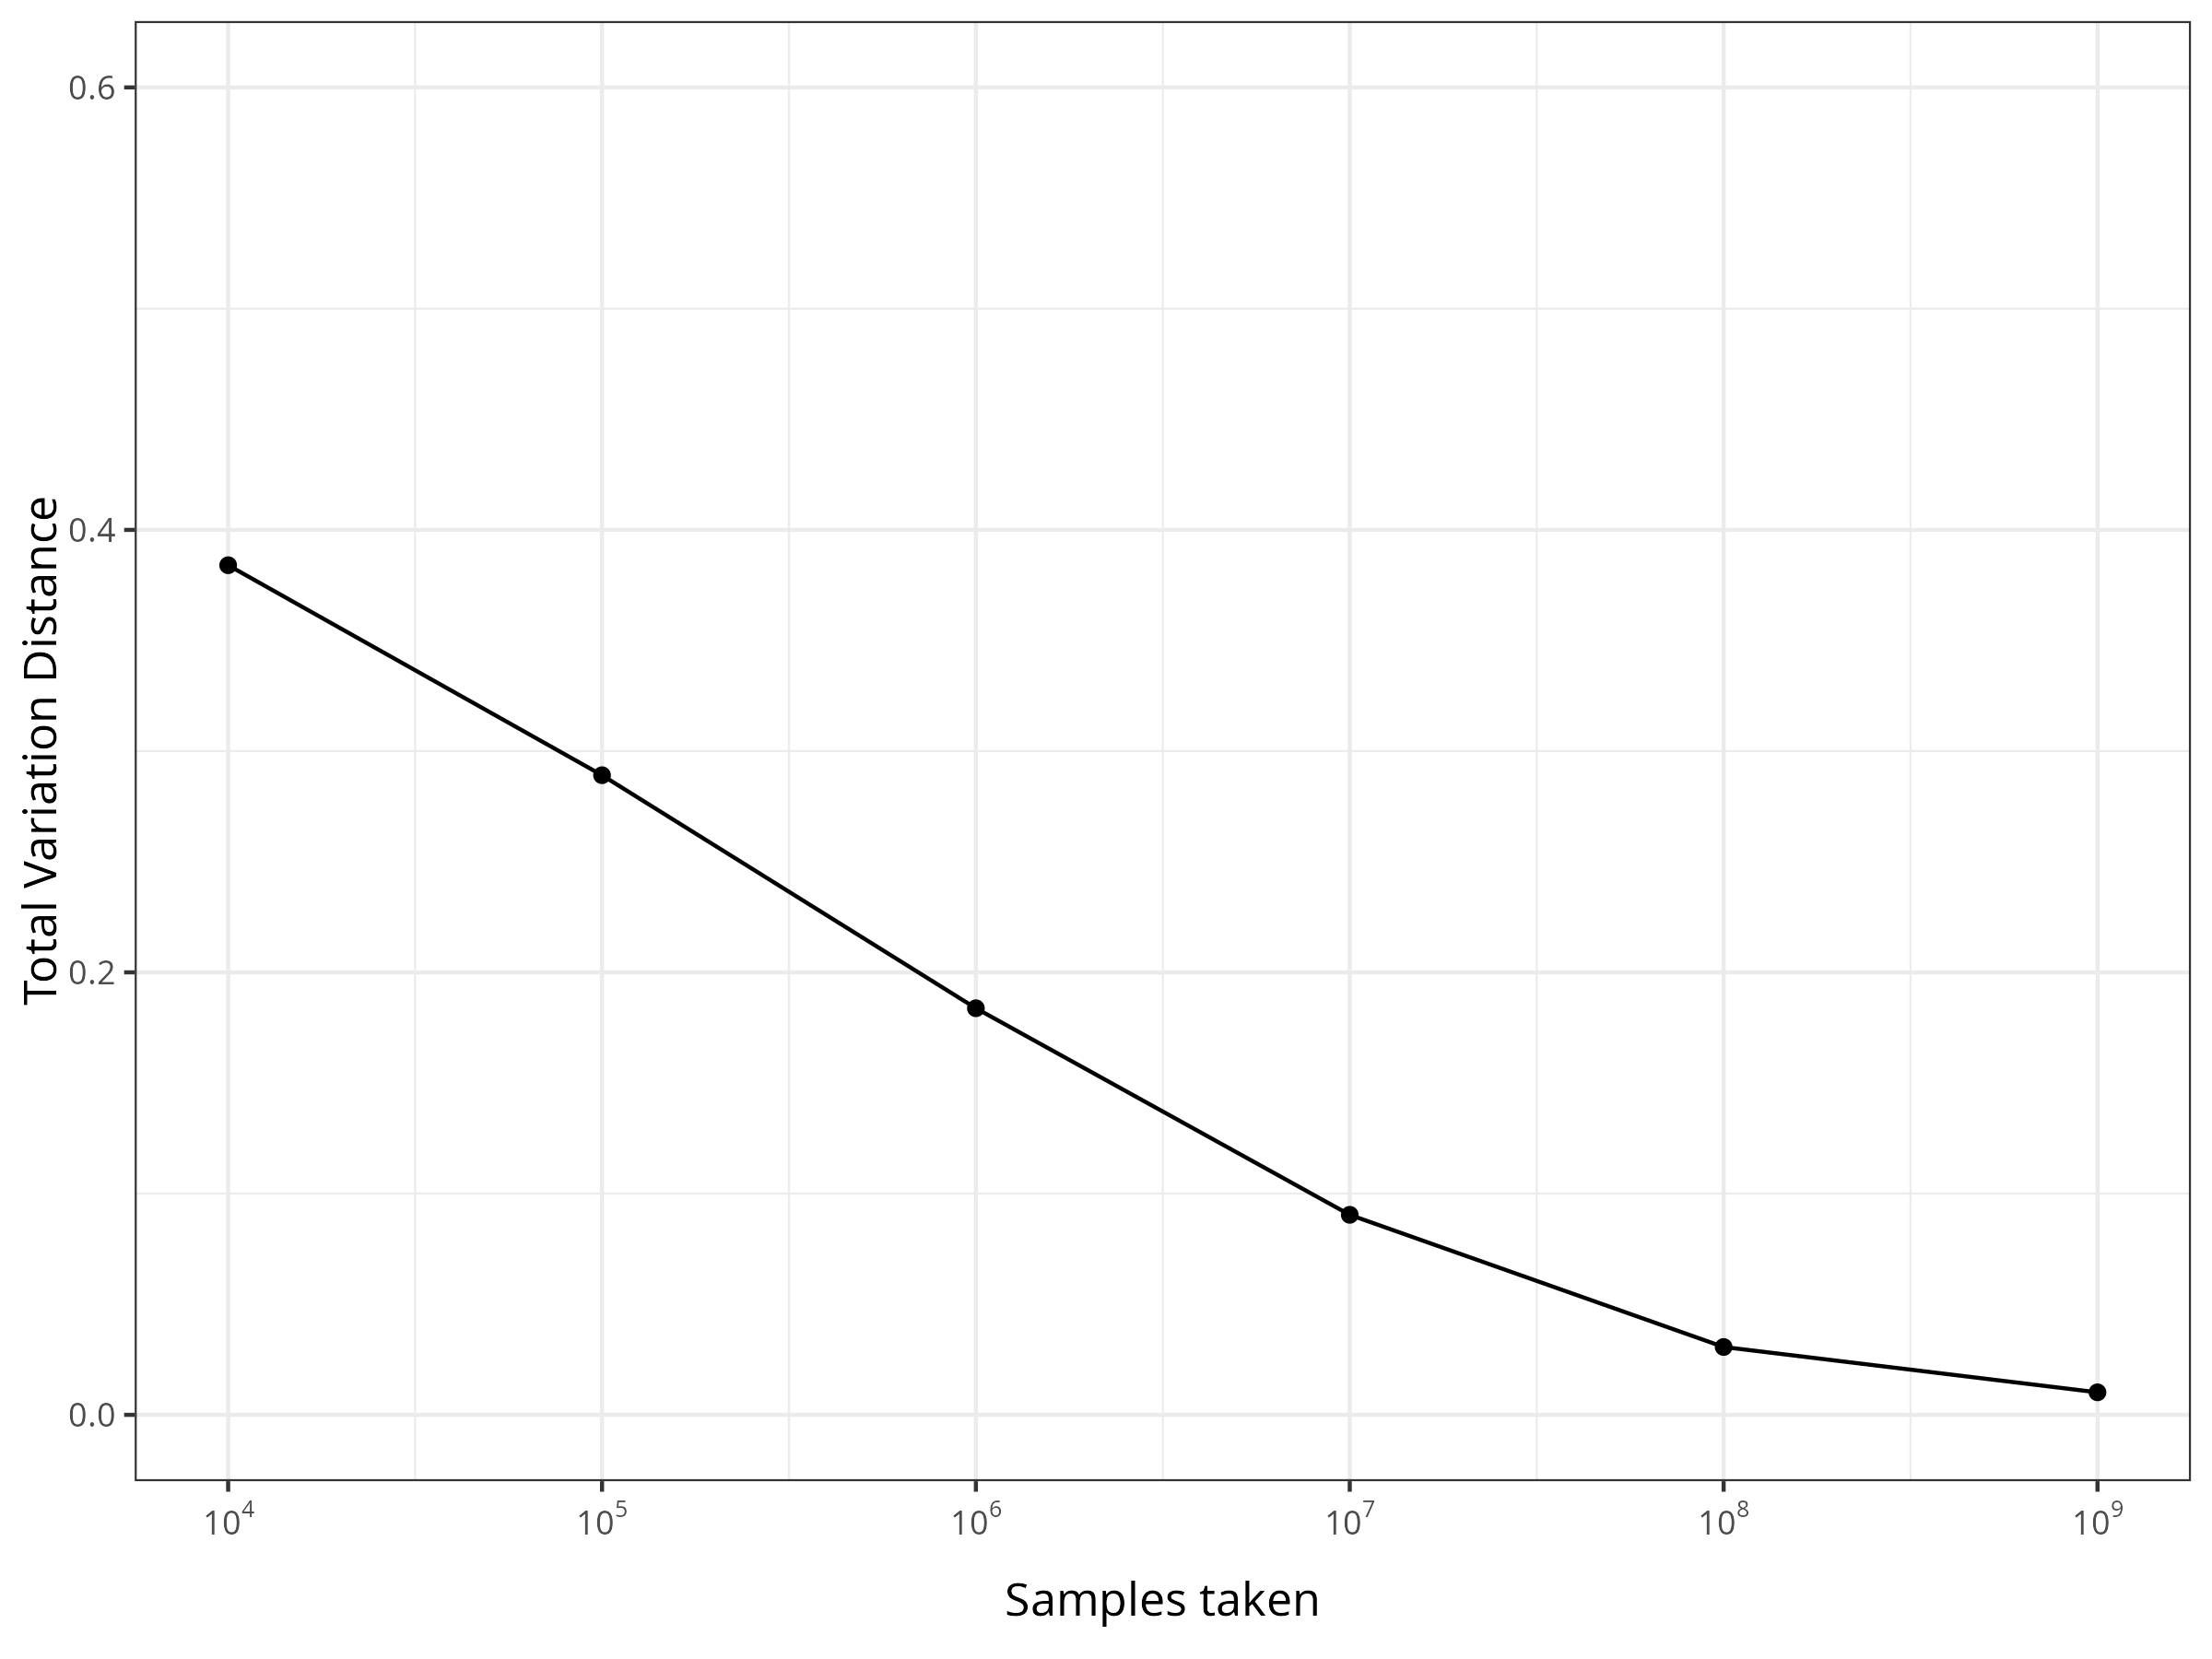
\includegraphics[width=\textwidth]{figures/tvd/ycsb.png}
        \caption{YCSB}
    \end{subfigure}
    
    \vspace{1em}

    % Second row
    \begin{subfigure}{0.46\textwidth}
        \centering
        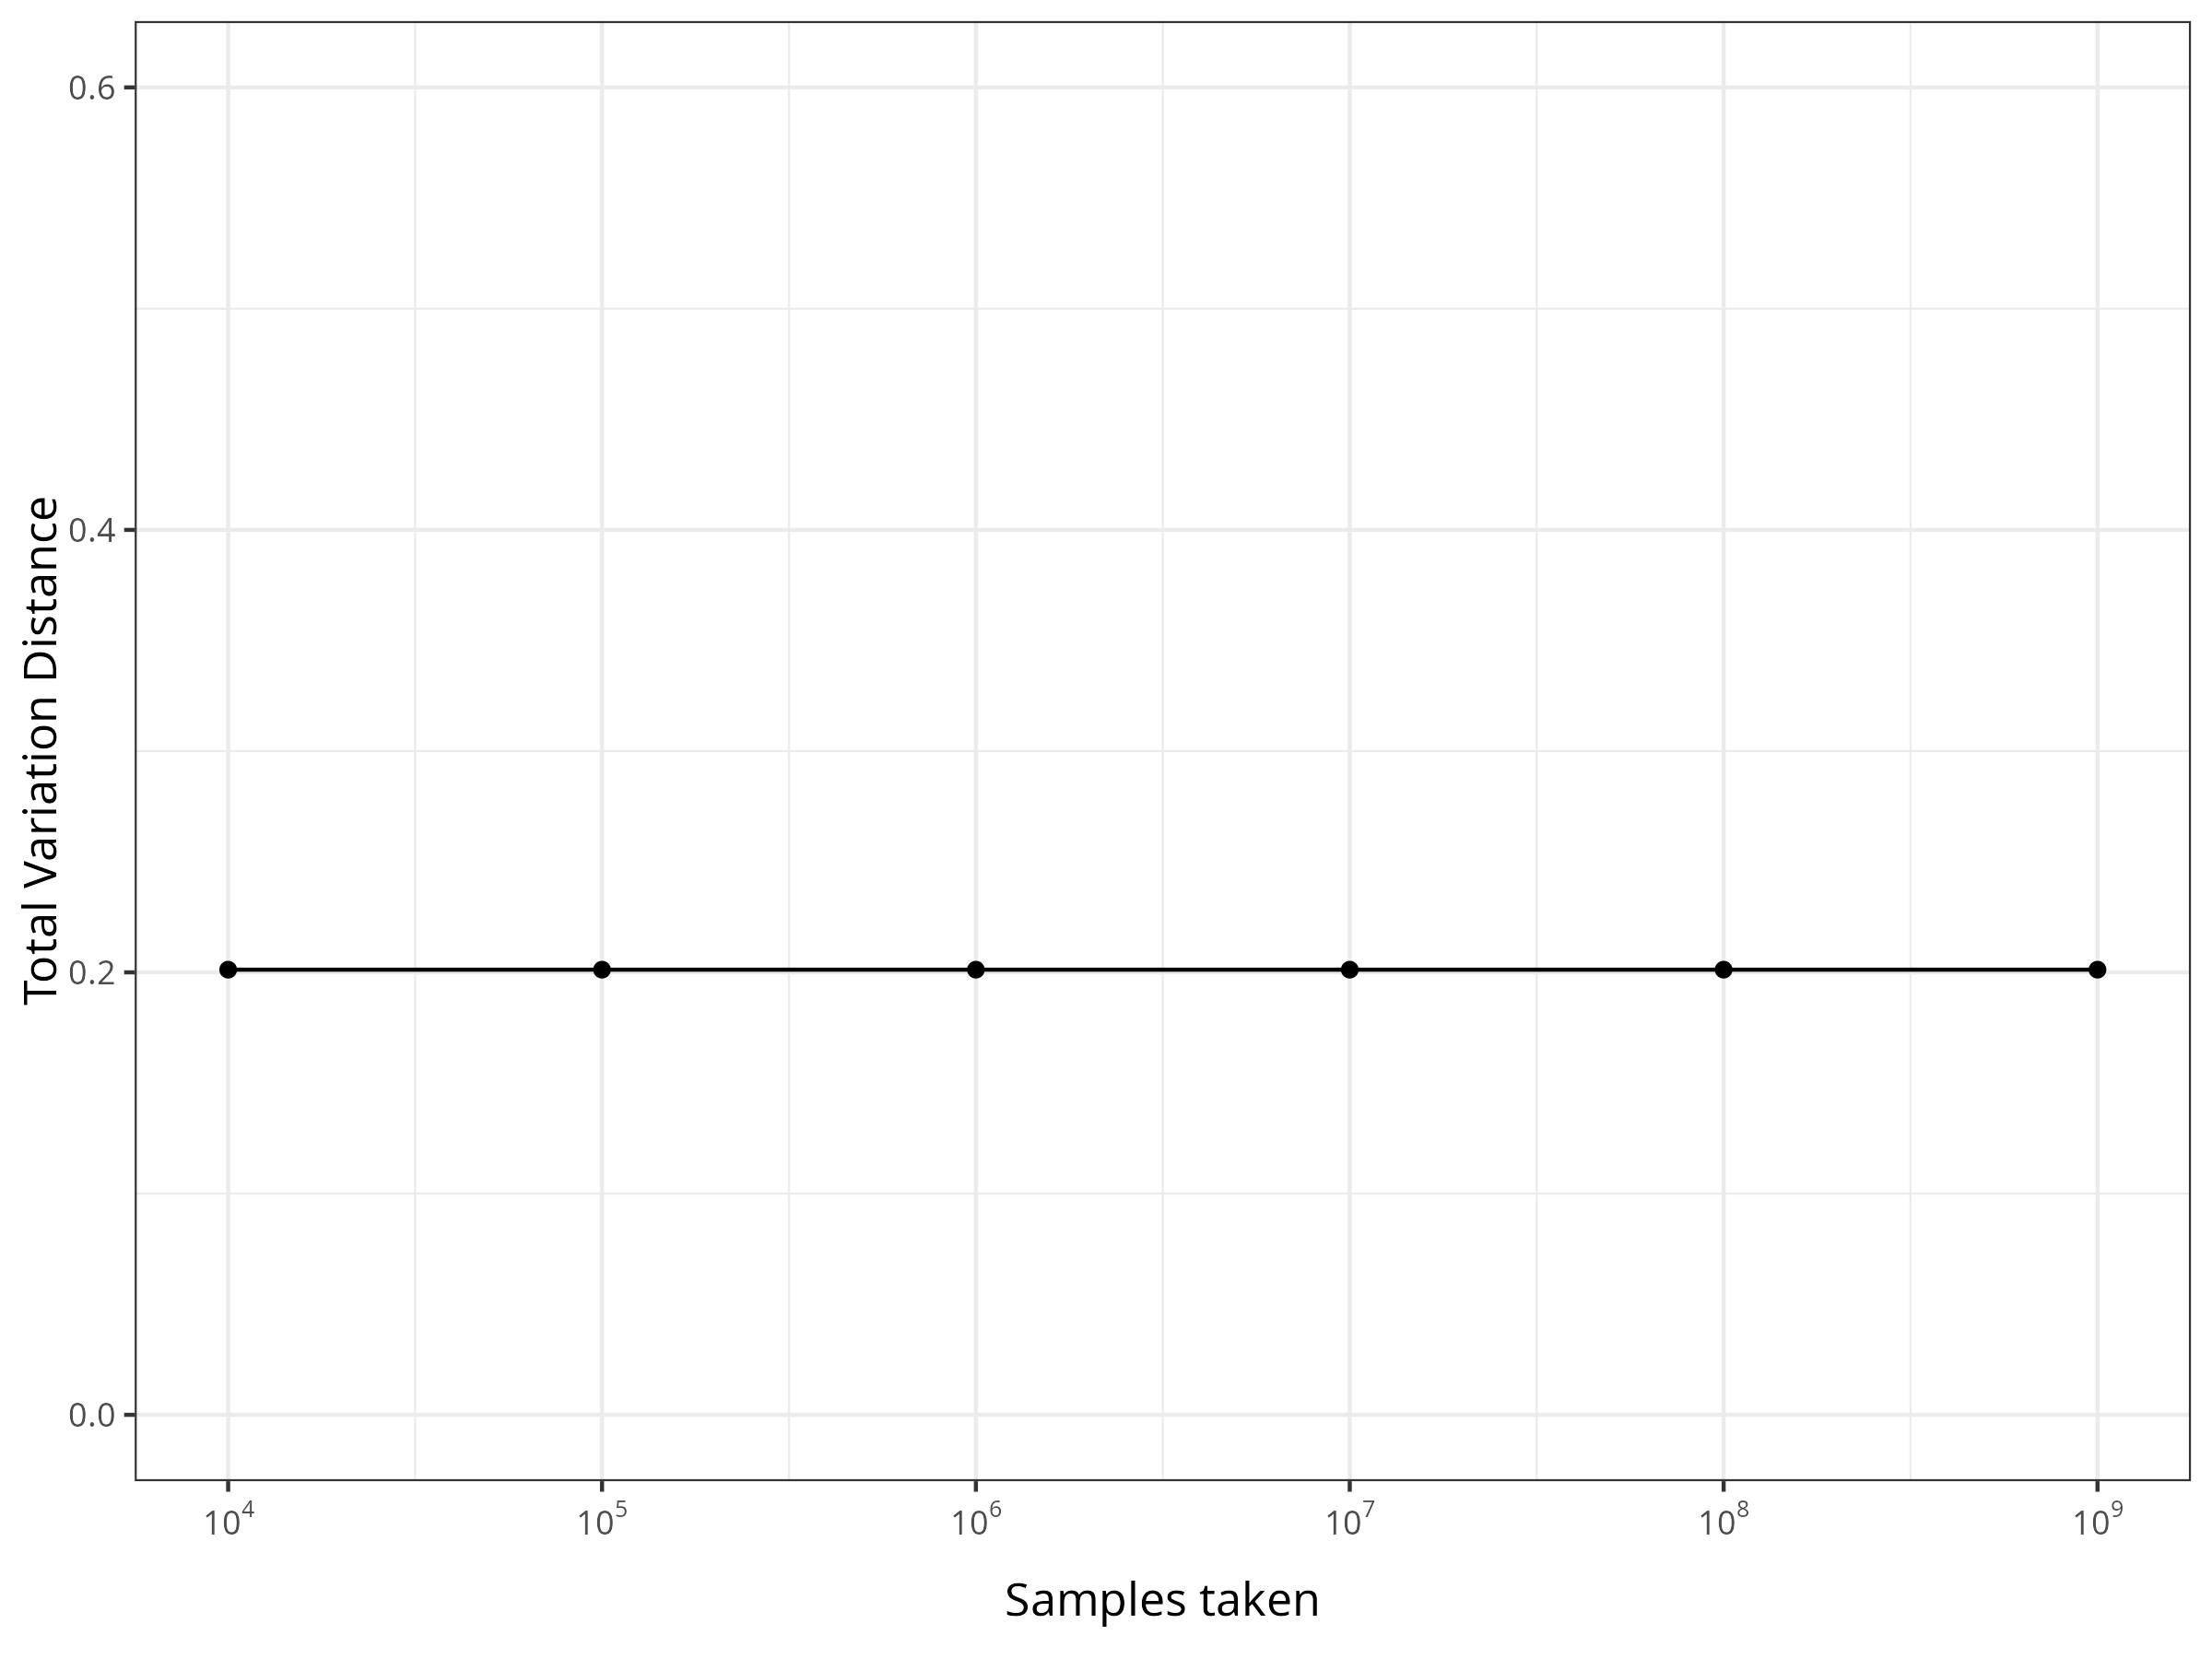
\includegraphics[width=\textwidth]{figures/tvd/fio.png}
        \caption{FIO}
    \end{subfigure}
    \hfill
    \begin{subfigure}{0.46\textwidth}
        \centering
        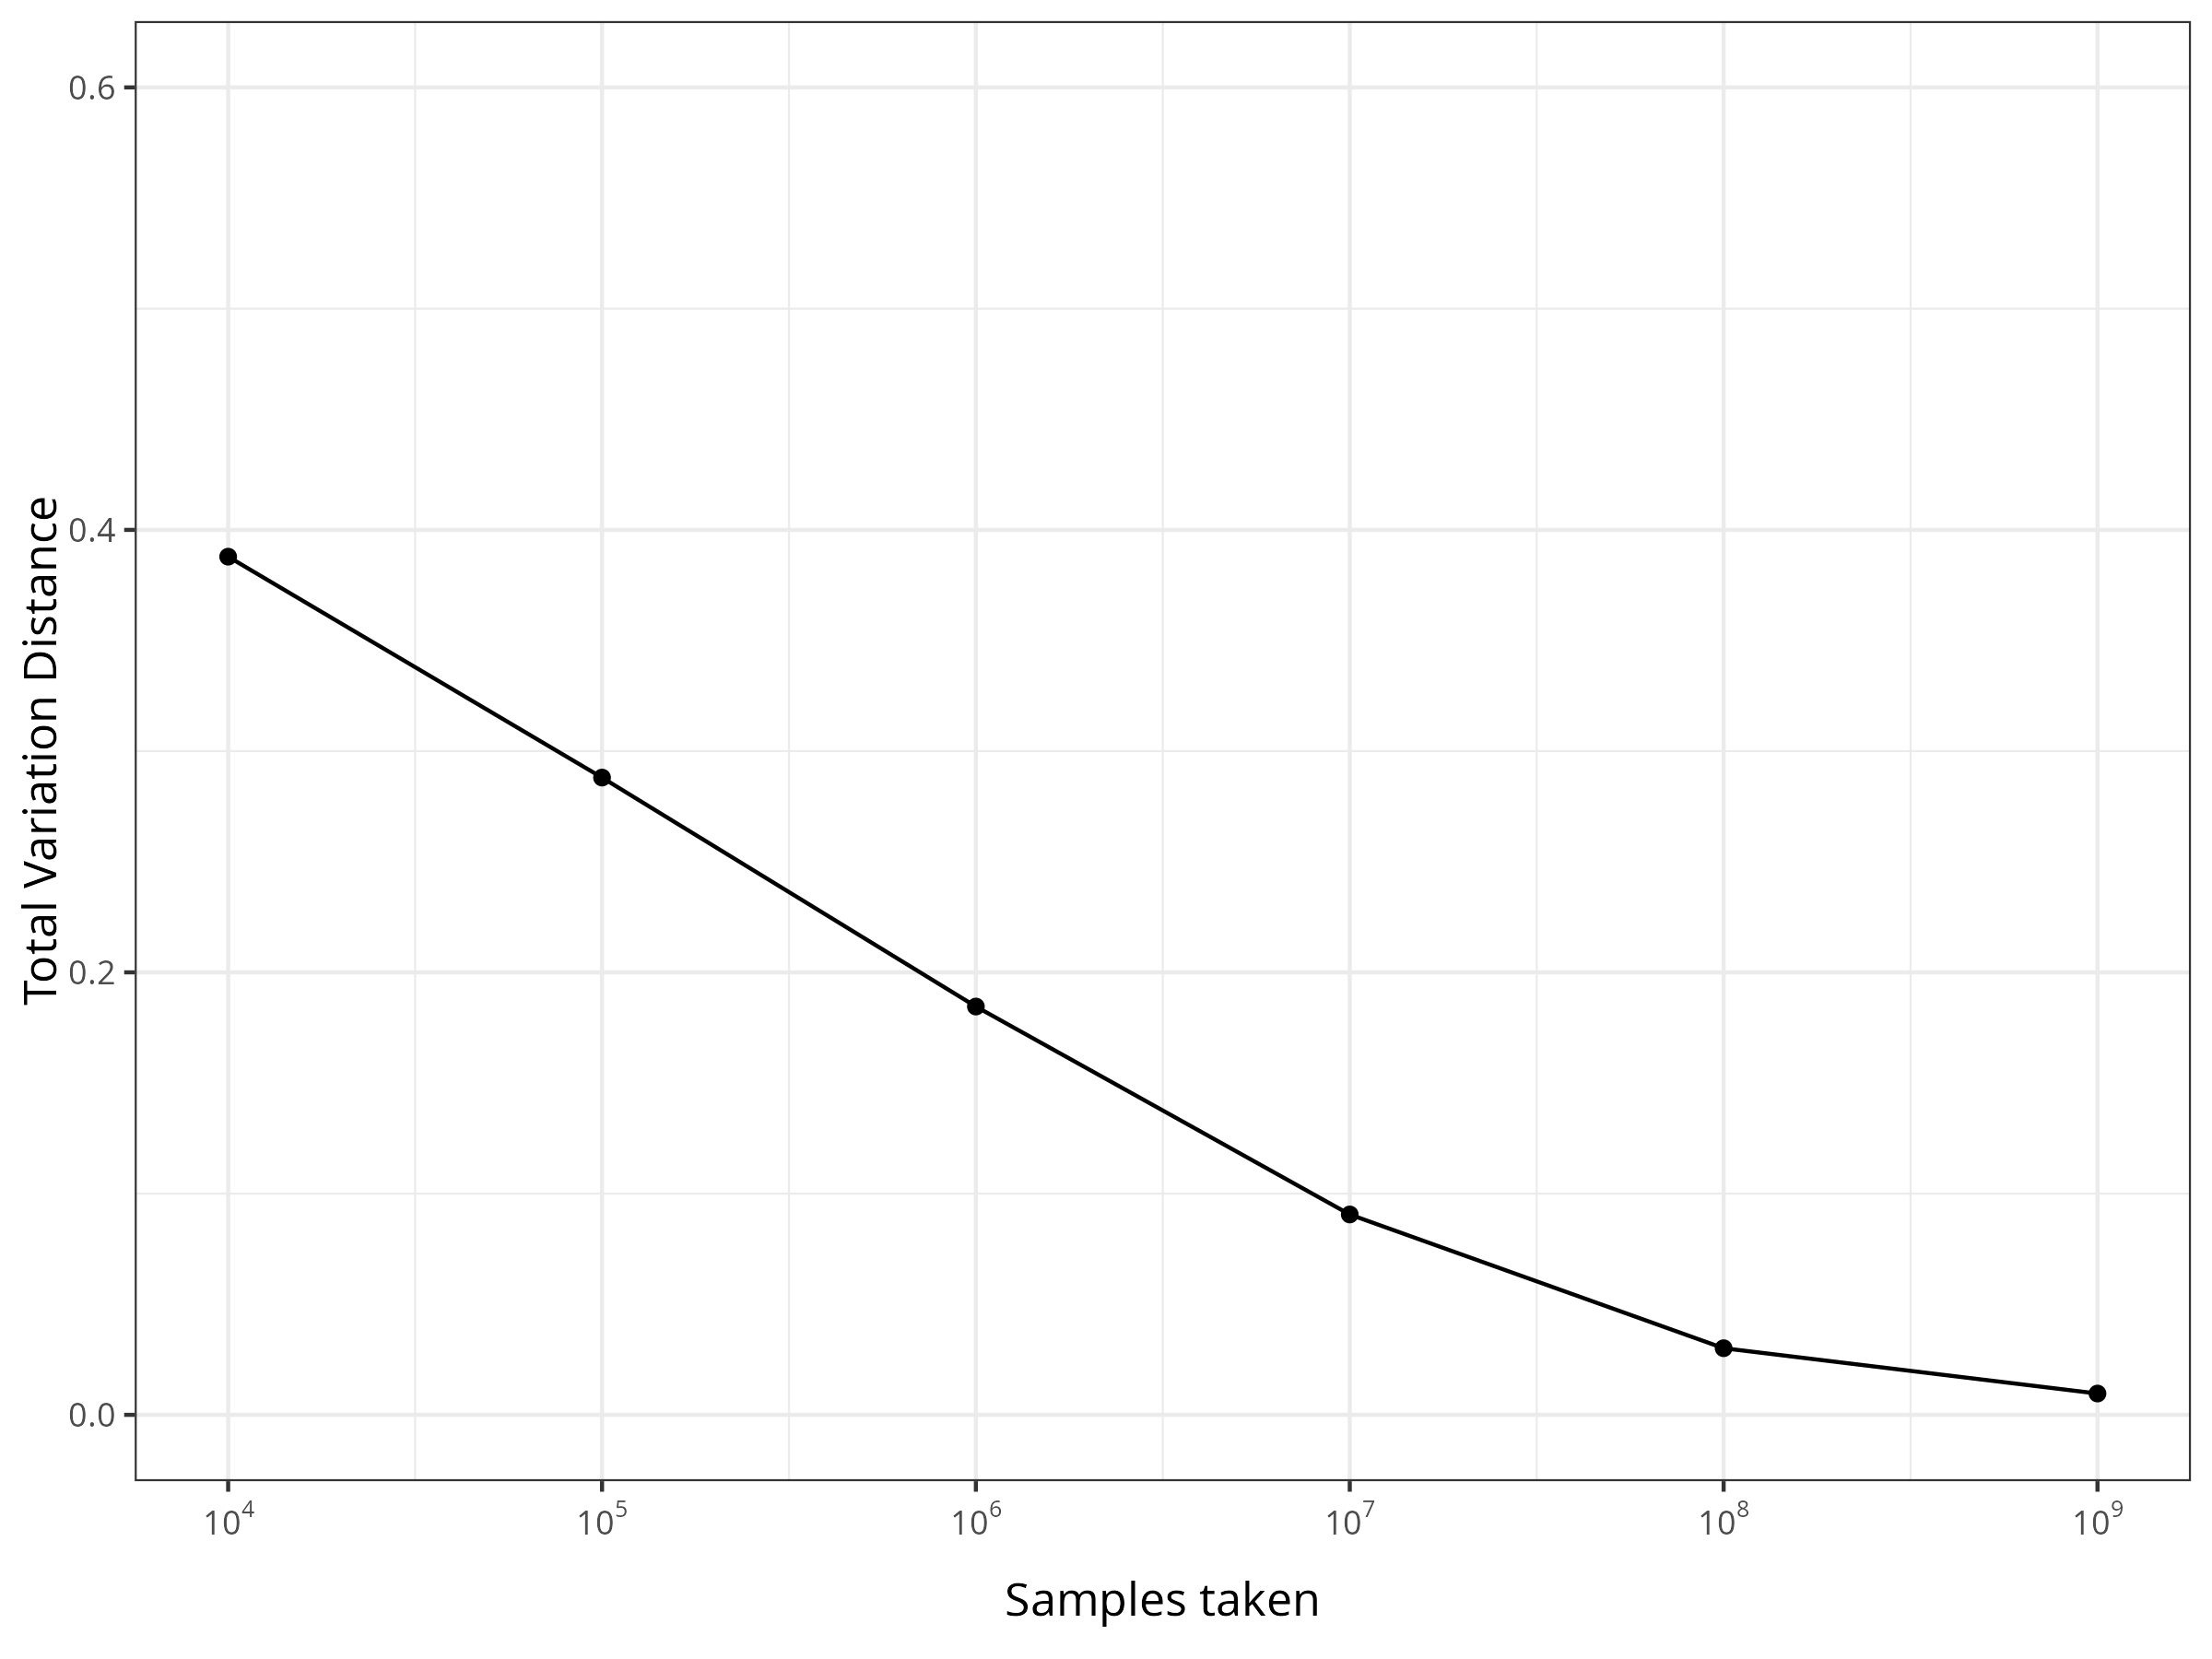
\includegraphics[width=\textwidth]{figures/tvd/sysbench.png}
        \caption{Sysbench}
    \end{subfigure}
    
    \vspace{1em}

    % Third row
    \begin{subfigure}{0.46\textwidth}
        \centering
        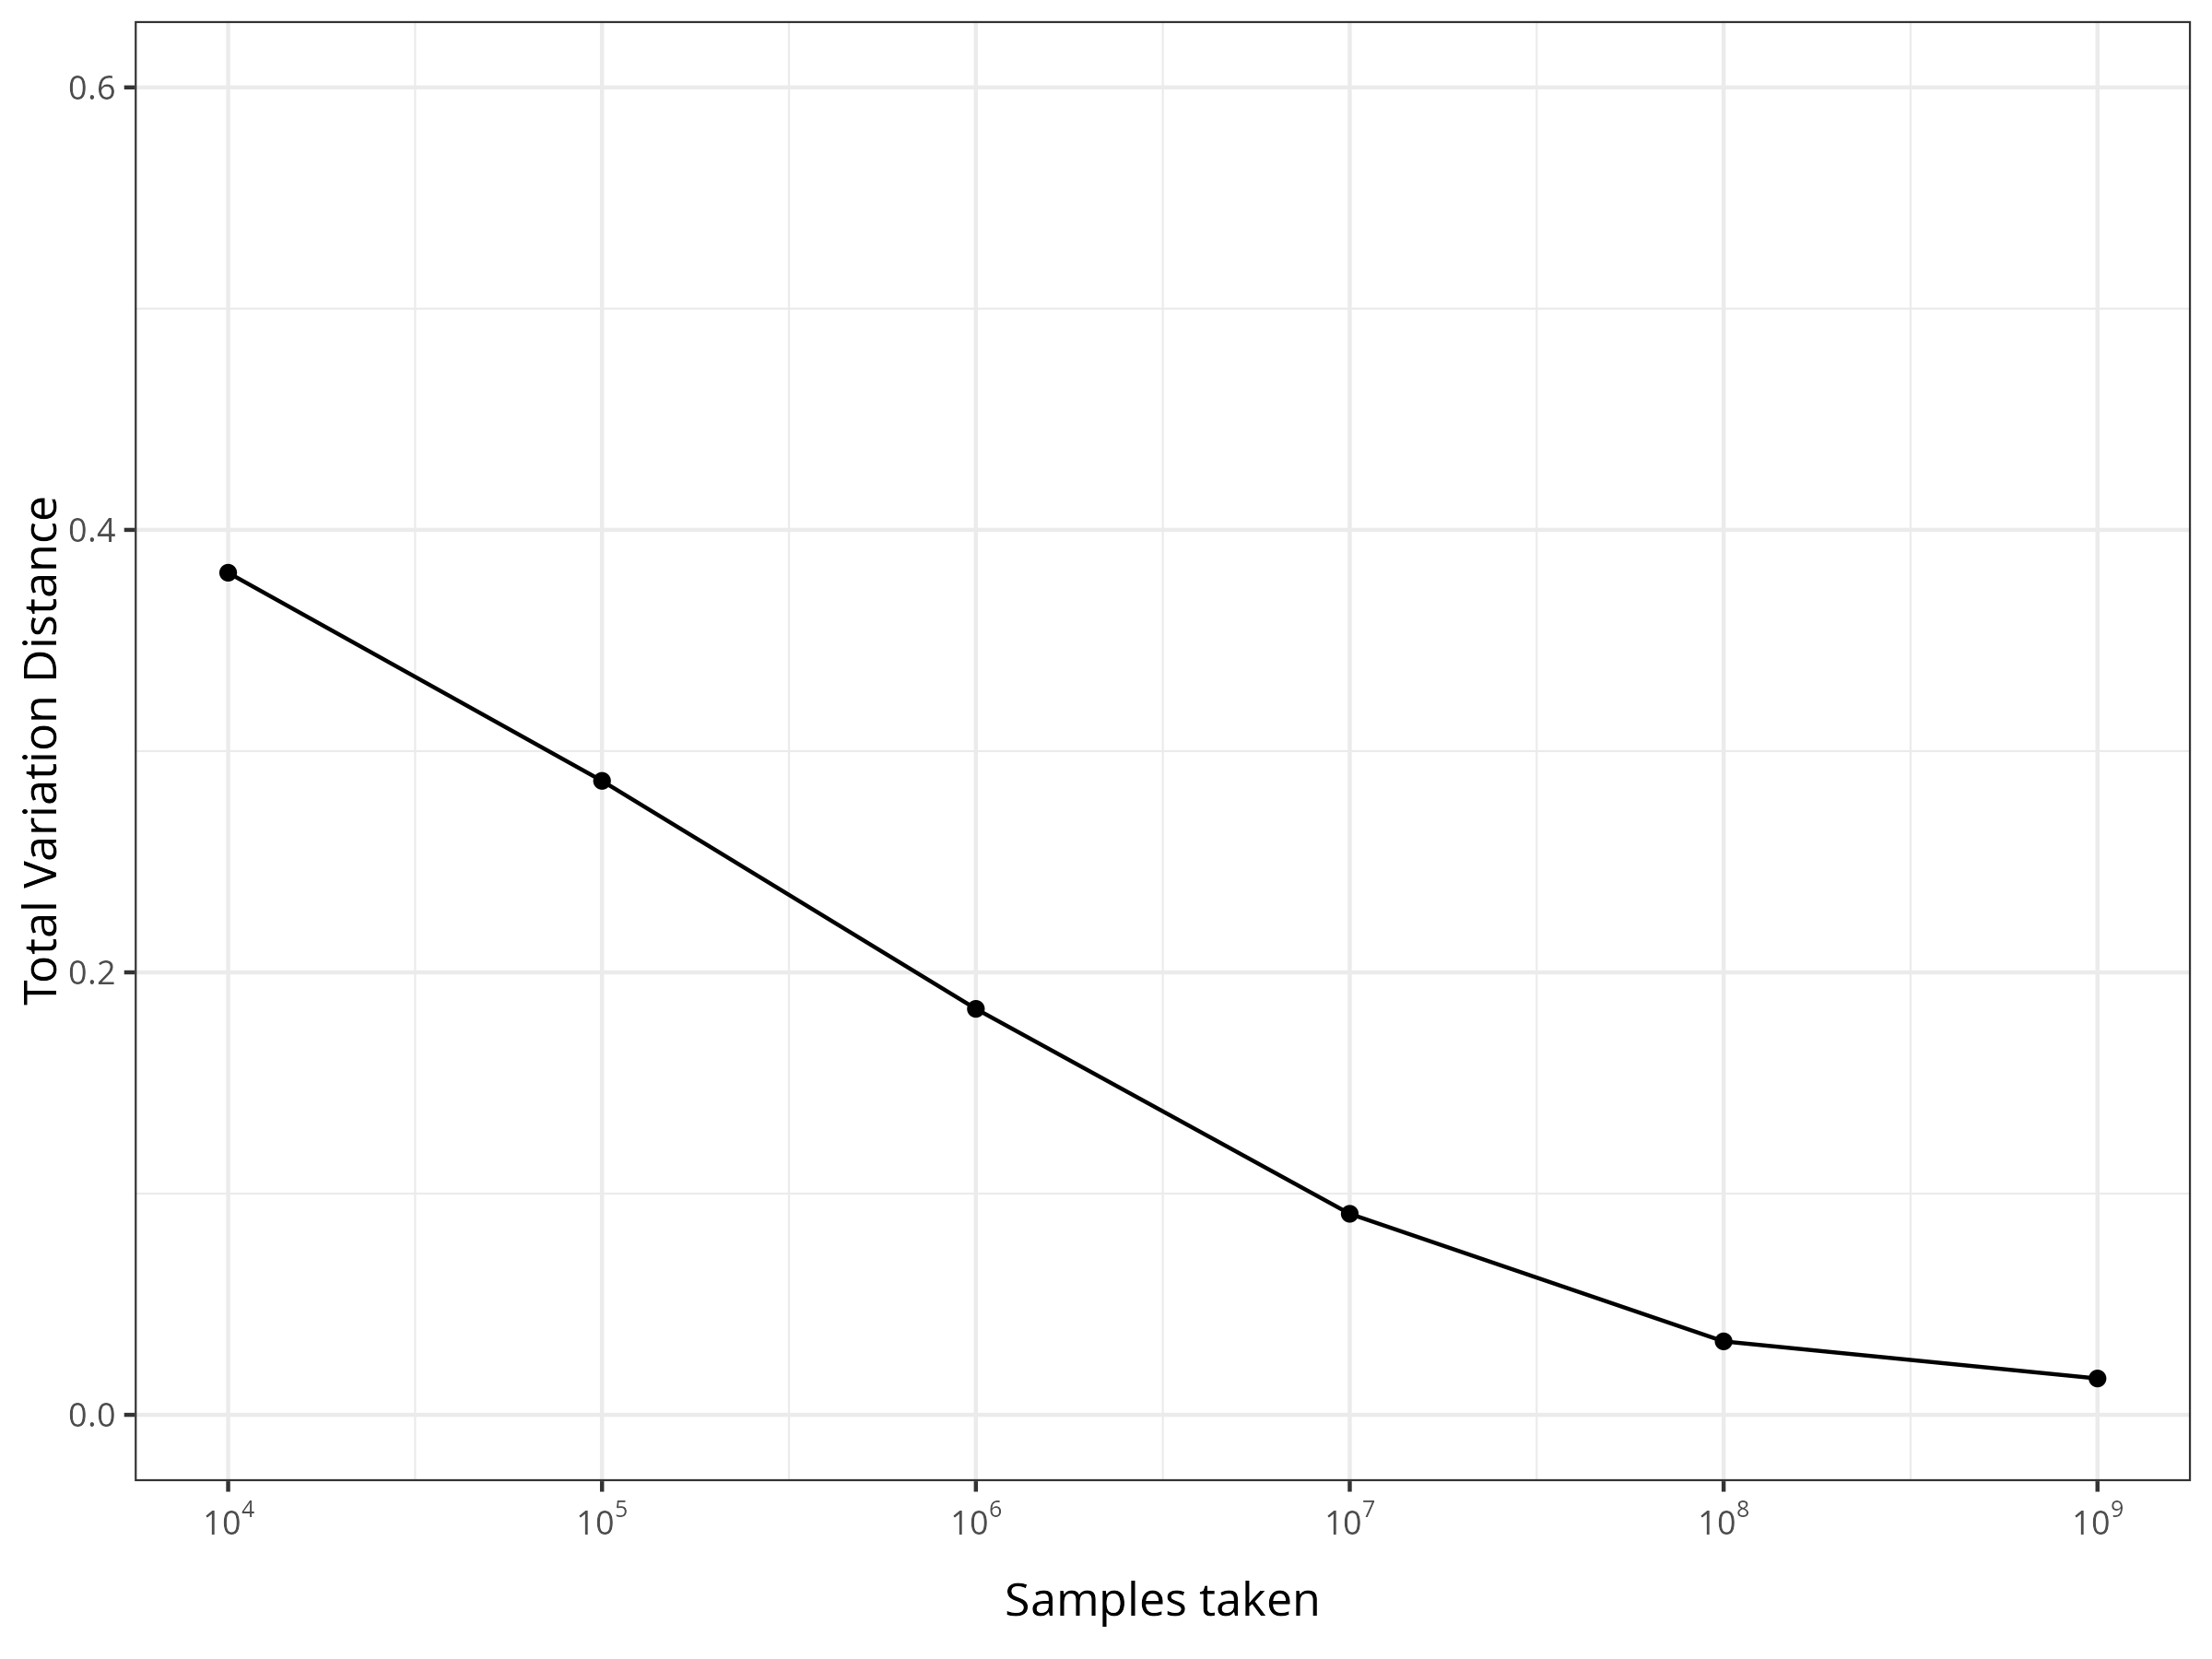
\includegraphics[width=\textwidth]{figures/tvd/marsaglia.png}
        \caption{Condensed Table Lookup}
    \end{subfigure}
    \hfill
    \begin{subfigure}{0.46\textwidth}
        \centering
        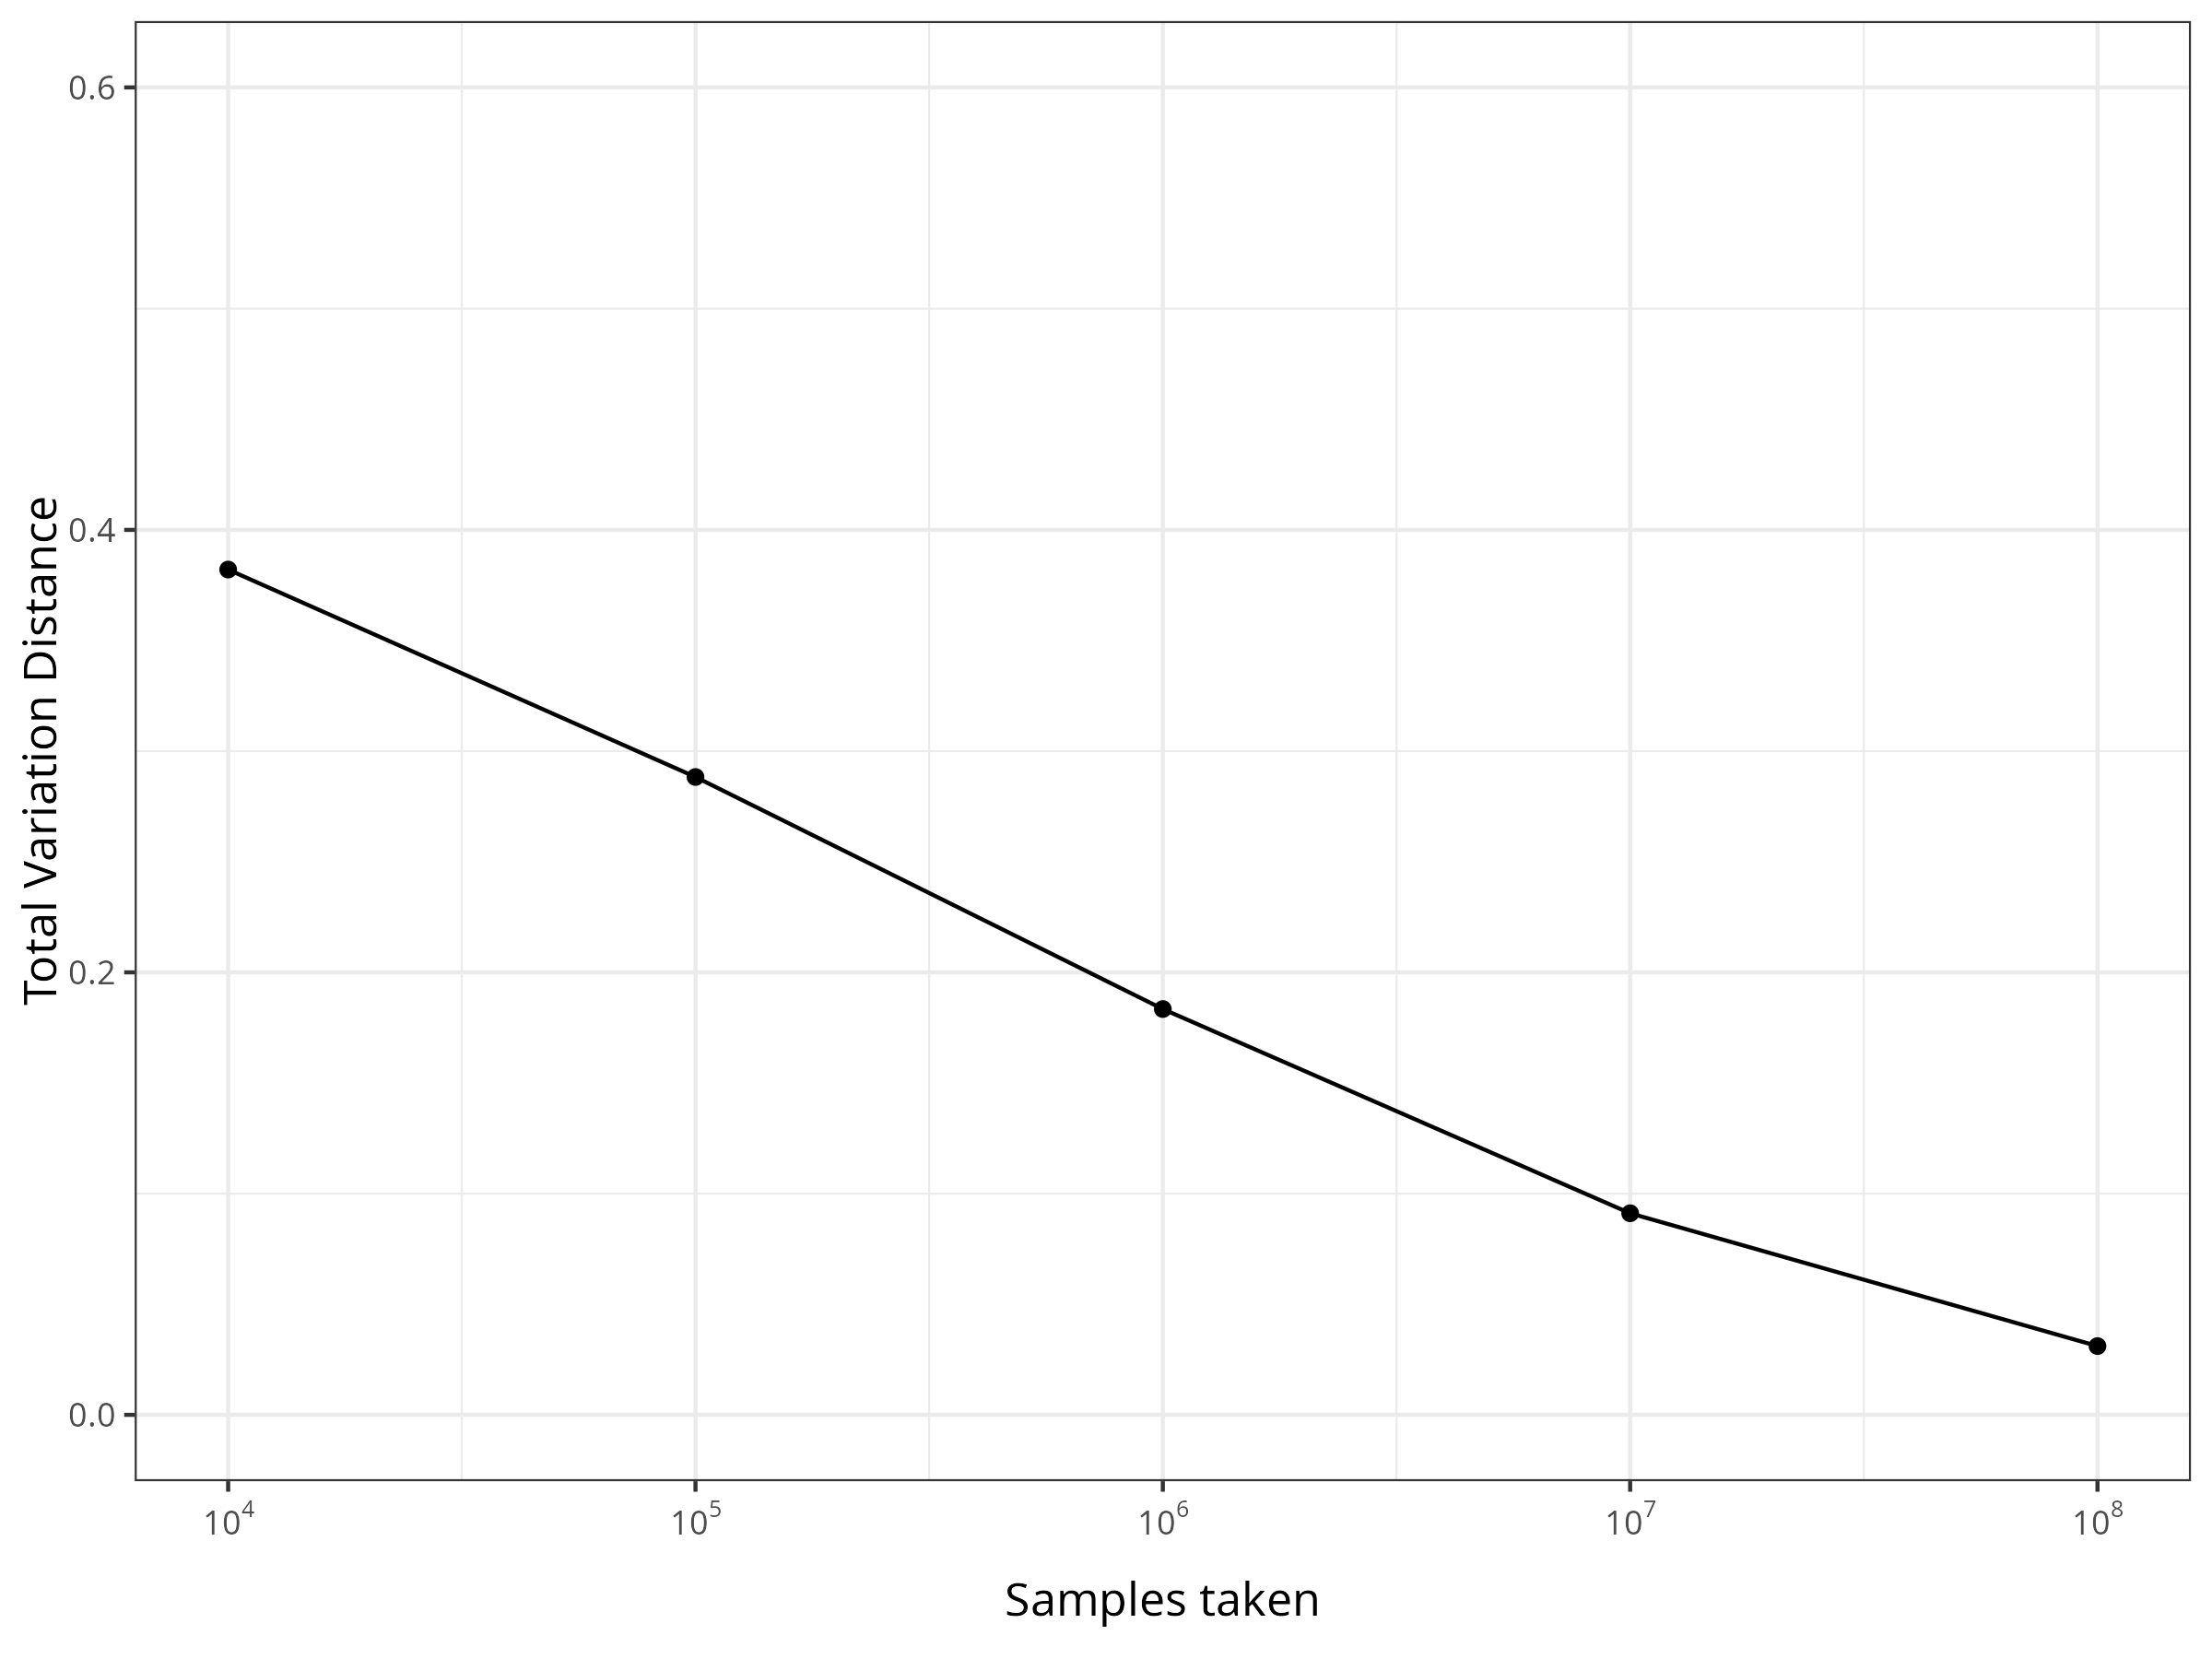
\includegraphics[width=\textwidth]{figures/tvd/rejection.png}
        \caption{Rejection Sampling}
    \end{subfigure}
    
    
    \caption{TVD test results for the different samplers.}
    \label{fig:tvd-graphs}
\end{figure}